
\section*{HS 1. feladat: Kazánfalon áthaladó hőmennyiség}
\addcontentsline{toc}{section}{HS 1. feladat}


\begin{tabular}{ | p{2cm} | p{14cm} | } 
	\hline
	Név & Kovács Bence \\ 
	\hline
	Szak &  Mechatronikai Mérnöki\\
	\hline
	Félév & 2019/2020 II. (tavaszi) félév \\ 
	\hline
\end{tabular}
\vspace{0.5cm}

Határozza meg azt a hőmennyiséget amely a kazánfal $\SI{1}{\meter^2}$-én óránként átadódik, ha a fal vastagsága $\SI{20}{\milli\meter}$, anyagának hővezetési tényezője $\SI{45}{\watt\per\meter}$ és a fal belső oldalát $\SI{2}{\milli\meter}$ vastag kazánkő réteg borítja. Ennek a hővezetési tényezője $\lambda = \SI{1.5}{\watt\per\meter\K}$ fok. A kazán falának füstgázoldali hőmérséklete $\SI{260}{\celsius}$, vízoldali hőmérséklete $\SI{195}{\celsius}$. Számítsa ki a kazán falának közepes hőmérsékletét és rajzolja fel a hőmérséklet-hely függvényt léptékhelyesen!
    \vspace{1mm}

Adatok: $\lambda_1 = \SI{45}{\watt\per\meter\K}$
        $\lambda_2 = \SI{1.5}{\watt\per\meter\K}$




\begin{equation}
	 {q} = \frac{\lambda_1}{\delta_1} (T_1 - T_2)
\end{equation}


\begin{equation}
	 {q}_1 = \frac{45}{0,02} (533,15 - T_2)
\end{equation}


\begin{equation}
	 {q}_2 = \frac{1,5}{0,002} (T_2 - 468,15)
\end{equation}


\begin{equation}     
     {q}_1 = \SI{2250}{\watt\per\K} \cdot (533,15 - T_2)
\end{equation}


 \begin{equation}   
    {q}_2 = \SI{750}{\watt\per\K}} \cdot (T_2 - 468,15)
\end{equation}

    
\begin{equation}    
    2250 \cdot (533,15-T_2) = 750(T_2-468.15)
\end{equation}


\begin{equation}
    1599,45-3 \cdot T_2 = T_2-468,15
\end{equation}
        

\begin{equation}
    T_2 = \frac{2067,6}{4} = \SI{516,9}{\Kelvin} = \SI{243,73}{\celsius}
\end{equation}
    
    
\begin{equation}
     {q} = \SI{750}{\watt\per\K}} \cdot (516,9 - 468,15) = \SI{36562,5}{\watt\per\meter^2} 
\end{equation}
    
\begin{equation}
     {T_k_o_z} = T_1- \frac{T_1 - T_2}{\delta_1} \cdot x
\end{equation}

\begin{equation}
     {T_k_o_z} = 533,15- \frac{533,15 - 516,9}{0,02} \cdot 0.01 = 525.025K = 251.87°C
\end{equation}
        
    \begin{figure}[h]
	\centering

		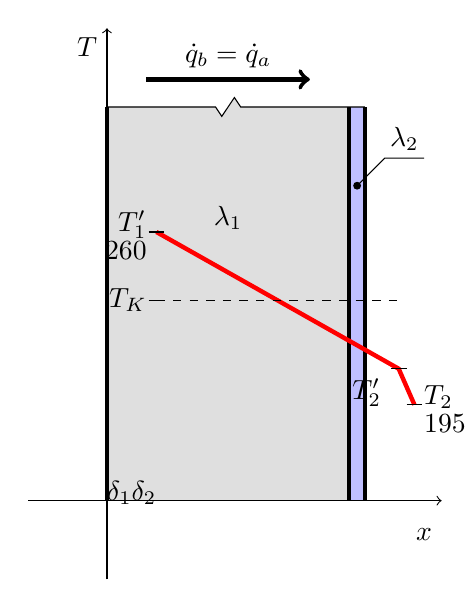
\begin{tikzpicture}
			\pgfmathsetmacro{\d}{20/6.5}
			\pgfmathsetmacro{\v}{1.2/6}
			\pgfmathsetmacro{\L}{5}
			\pgfmathsetmacro{\TA}{260/160*2.1}
			\pgfmathsetmacro{\TB}{243.73/160*1.1}
			\pgfmathsetmacro{\TC}{195/160}
			\pgfmathsetmacro{\TK}{(\TA+\TB)/2}
			
			% Fal
			\fill[gray,opacity=0.25] (0,0) -- (0,\L) -- ({\d/2-0.16},\L) -- ({\d/2-0.08}, {\L-0.12}) -- ({\d/2+0.08}, {\L +0.12}) -- ({\d/2+0.16}, \L) -- (\d, \L) -- (\d, 0);
			\fill[blue,opacity=0.25] (\d, \L) -- (\d, 0) -- (\d+\v, 0) -- (\d+\v, \L);
			\draw[] (0,\L) -- ({\d/2-0.16},\L) -- ({\d/2-0.08}, {\L-0.12}) -- ({\d/2+0.08}, {\L+0.12}) -- ({\d/2+0.16}, \L) -- (\d, \L) -- (\d+\v, \L);
			\draw[ultra thick] (0,0) -- (0,\L);
			\draw[ultra thick] (\d, 0) -- (\d, \L);
			\draw[ultra thick] (\d+\v, 0) -- (\d+\v, \L);
			
			% Tengelyek
			\draw[->] (0,-1) -- (0,\L+1) node[anchor=north east]{$T$};
			\draw[->] (-1,0) -- (4.25,0) node[anchor=base east, shift={(0,-0.5)}]{$x$};
			
			% Hőáram és hőáramsűrűség
			\draw[->, ultra thick] (0.5,{\L+0.35}) -- ({\d/2},{\L+0.35}) node[anchor=south]{$\dot{q}_b = \dot{q}_a$} -- ({\d - 0.5},{\L+0.35});
			
			% A hővezetési tényező
			\node[anchor=base] at ({\d/2},{\L-1.5}) {$\lambda_1$};
			\node[anchor=base] at ({\d+\v+0.5},{\L-0.5}) {$\lambda_2$};
			\draw ({\d+\v+0.75},{\L-0.65}) -- ({\d+\v+0.25},{\L-0.65}) -- ({\d+\v/2},{\L-1});
			\fill[] ({\d+\v/2},{\L-1}) circle[radius=0.05];
			
			% A falvastagságok
			\pgflength[xa=0, ya=0, xb=\d, yb=0, alim=0]{$\delta_1$};
			\pgflength[xa=\d, ya=0, xb=\d+\v, yb=0, alim=0, a=0, belül=2]{$\delta_2$};
			
			% T(x)
			\draw[red, ultra thick] (0,\TA) -- (\d,\TB) -- (\d+\v,\TC);
			
			% Falhőmérsékletek
			\draw (-0.1,\TA) -- (0.1,\TA);
			\node[anchor=base east] at (0,\TA) {$T_1'$};
			
			\draw (-0.1+\d,\TB) -- (0.1+\d,\TB);
			\node[anchor=north east] at (\d-0.1,\TB) {$T_2'$};
			
			\node[anchor=north east] at (0,\TA) {$\SI{260}{\celsius}$};
			
			\draw (-0.1+\d+\v,\TC) -- (0.1+\d+\v,\TC);
			\node[anchor=base west] at (\d+\v,\TC) {$T_2$};
			\node[anchor=north west] at (\d+\v,\TC) {$\SI{195}{\celsius}$};
			
			% A közepes hőmérséklet
			\draw[dashed] (0,\TK) -- (\d,\TK);
			\draw (-0.1,\TK) -- (0.1,\TK);
			\node[anchor=east] at (0,\TK) {$T_K$};
			
		\end{tikzpicture}
		\caption{Hőmérséklet-hely függvény}

\end{figure}
